\documentclass[12pt]{article}
\usepackage[utf8]{inputenc}
\usepackage[T1]{fontenc}
\usepackage[spanish,es-lcroman]{babel}
\usepackage{amsmath}
\usepackage{amsthm}
\usepackage{physics}
\usepackage{tikz}
\usepackage{float}
\usepackage{cancel}
\usepackage[autostyle,spanish=mexican]{csquotes}
\usepackage[per-mode=symbol]{siunitx}
\usepackage{gensymb}
\usepackage{multicol}
\usepackage{enumitem}
\usepackage{stackengine}
\usepackage{stix}
\usepackage[left=2.00cm, right=2.00cm, top=2.00cm, 
     bottom=2.00cm]{geometry}

\usepackage{Estilos/ColoresLatex}
\usepackage{makecell}
\usepackage{wrapfig}
% \usepackage{titlesec}
\usetikzlibrary{angles,quotes}
\newcommand{\sectionbreak}{\clearpage}

\newcommand{\textocolor}[2]{\textbf{\textcolor{#1}{#2}}}
%\renewcommand{\questionlabel}{\thequestion)}

\newcommand{\Cancel}[2][black]{{\color{#1}\cancel{\color{black}#2}}}

\newcommand\deci[1]{%
    \kern-.4ex\stackunder[0.4pt]{$#1$}{$\color{blue}\acwunderarcarrow$}
}

\newcommand\decposl[1]{%    <--- Decimal position to left
    \kern-.4ex\stackunder[0.4pt]{$#1$}{%
      \reflectbox{$\color{red}\kern-.6ex\acwunderarcarrow$}
      }
}

\decimalpoint
\sisetup{bracket-numbers = false}

\title{\vspace*{-2cm} Sustentabilidad y contaminación}
\author{M. en C. Ramón Gustavo Contreras Mayén \\ {\fontsize{14}{14}\selectfont Universidad del Valle de México. Campus San Rafael}}
% \institute{Universidad del Valle de México. Campus San Rafael.}
\date{}

\begin{document}
\maketitle

\section{Sustentabilidad.}

La sustentabilidad se refiere a la capacidad de satisfacer las necesidades presentes sin comprometer la capacidad de las futuras generaciones para satisfacer sus propias necesidades. Implica equilibrar los aspectos económicos, sociales y ambientales para garantizar un desarrollo sostenible a largo plazo. Mencionamos a continuación algunos puntos clave sobre la sustentabilidad:
\begin{enumerate}
\item \textbf{Aspecto ambiental}:

La sustentabilidad ambiental se enfoca en proteger y conservar los recursos naturales, así como en mitigar los impactos negativos sobre el medio ambiente. Esto incluye la reducción de la contaminación, la conservación de la biodiversidad, el uso eficiente de los recursos naturales y la lucha contra el cambio climático.
\item \textbf{Aspecto social}:

La sustentabilidad social se relaciona con la equidad, la justicia social y el bienestar humano. Busca garantizar que todas las personas tengan acceso a recursos básicos como agua limpia, alimentos, vivienda, educación y atención médica. También se enfoca en promover la inclusión, la igualdad de género, el respeto a los derechos humanos y la participación ciudadana en la toma de decisiones.
\item \textbf{Aspecto económico}:

La sustentabilidad económica implica el desarrollo de una economía próspera y equitativa que satisfaga las necesidades de las personas sin comprometer los recursos naturales ni el bienestar de las generaciones futuras. Se centra en promover la eficiencia económica, la innovación tecnológica, la creación de empleo decente y el acceso equitativo a oportunidades económicas.
\item \textbf{Enfoque de ciclo de vida}:

La sustentabilidad adopta un enfoque de ciclo de vida en todas las actividades humanas, considerando los impactos ambientales, sociales y económicos desde la extracción de materias primas hasta la disposición final de los productos. Esto implica la reducción de residuos, la reutilización y el reciclaje de materiales, así como la promoción de prácticas comerciales éticas y responsables.
\item \textbf{Colaboración y cooperación}:

La sustentabilidad requiere la colaboración y cooperación entre diferentes actores, incluyendo gobiernos, empresas, organizaciones no gubernamentales y la sociedad civil. Es necesario establecer alianzas y trabajar juntos para abordar los desafíos globales y promover un desarrollo sustentable en todas sus dimensiones.
\end{enumerate}

\section{Física y contaminación.}

La física desempeña un papel importante en el estudio, la comprensión y la mitigación de la contaminación en sus diversas formas. Revisemos a continuación, algunas formas en que la física contribuye al análisis y la gestión de la contaminación:
\begin{enumerate}
\item \textbf{Estudio de la dispersión de contaminantes}:

La física proporciona modelos matemáticos y herramientas computacionales para predecir cómo se dispersan los contaminantes en la atmósfera, el agua y el suelo. Estos modelos se basan en principios físicos como la difusión, la convección y la advección, y ayudan a los científicos y los gestores del medio ambiente a comprender la dinámica de los contaminantes y a tomar medidas adecuadas para su control.
\item \textbf{Monitoreo de la contaminación}:

La física ofrece una variedad de técnicas y dispositivos para medir la concentración de contaminantes en el aire, el agua y el suelo. Esto incluye instrumentos como espectrómetros, sensores remotos, cromatógrafos y detectores de partículas. Estos instrumentos permiten a los científicos y a las agencias ambientales realizar un seguimiento de la calidad del medio ambiente y evaluar el cumplimiento de los estándares de calidad del aire y del agua.
\item \textbf{Tratamiento de residuos y contaminantes}:

La física también se utiliza en el diseño y la operación de tecnologías para el tratamiento de residuos y contaminantes. Esto incluye procesos como la filtración, la destilación, la oxidación, la adsorción y la fotocatálisis, que se basan en principios físicos para eliminar los contaminantes del aire y el agua.
\item \textbf{Energías renovables}:

La contaminación del aire y del agua está estrechamente relacionada con la quema de combustibles fósiles y la generación de energía. La física desempeña un papel importante en el desarrollo y la implementación de tecnologías de energía renovable, como la energía solar, eólica, hidroeléctrica y geotérmica, que tienen un menor impacto ambiental y contribuyen a reducir las emisiones de gases de efecto invernadero.
\item \textbf{Educación y conciencia pública}:

La física proporciona la base científica necesaria para educar al público sobre los problemas de contaminación y promover la adopción de prácticas y políticas ambientales sostenibles.
\end{enumerate}
Comprender los principios físicos detrás de la contaminación puede ayudar a las personas a tomar decisiones informadas sobre su impacto en el medio ambiente y a buscar soluciones para reducir su huella ecológica.

\section{Día Internacional de la Madre Tierra.}

El Día Internacional de la Madre Tierra se celebra el 22 de abril de cada año como un recordatorio de la importancia de cuidar y proteger nuestro planeta. Fue establecido por la Asamblea General de las Naciones Unidas en 2009 con el objetivo de crear conciencia sobre los desafíos ambientales que enfrentamos y la necesidad de promover la sustentabilidad.

El Día de la Madre Tierra busca recordarnos que el planeta en el que vivimos es nuestro hogar común y que todos tenemos la responsabilidad de protegerlo y preservarlo para las generaciones futuras. Se centra en promover la armonía con la naturaleza y en adoptar prácticas sostenibles en nuestras vidas diarias.

Cada año, el Día de la Madre Tierra tiene un tema específico que destaca un aspecto particular de la protección del medio ambiente. Las actividades relacionadas con este día incluyen campañas de limpieza, siembra de árboles, eventos educativos sobre temas ambientales, conferencias y actividades comunitarias orientadas a promover la conservación y el cuidado de la Tierra.

El Día Internacional de la Madre Tierra nos recuerda que todos somos parte de un sistema interconectado y que nuestras acciones individuales pueden tener un impacto significativo en la salud y el bienestar del planeta. Es una oportunidad para reflexionar sobre nuestro papel como guardianes de la Tierra y para comprometernos a tomar medidas concretas para protegerla y preservarla.

\section{Efecto invernadero.}
\subsection{¿Qué es el efecto invernadero?}

El efecto invernadero es un proceso natural y esencial para mantener la temperatura de la Tierra en niveles adecuados para la vida.

Este fenómeno ocurre cuando ciertos gases en la atmósfera terrestre, conocidos como gases de efecto invernadero (GEI), absorben y emiten radiación infrarroja. Lo que provoca que parte del calor emitido por la superficie terrestre sea retenido y reenviado de vuelta a la superficie.

Esto crea un efecto similar al que se observa en un invernadero, donde el vidrio permite que la luz solar entre pero impide que el calor se escape.
\begin{figure}[H]
    \centering
    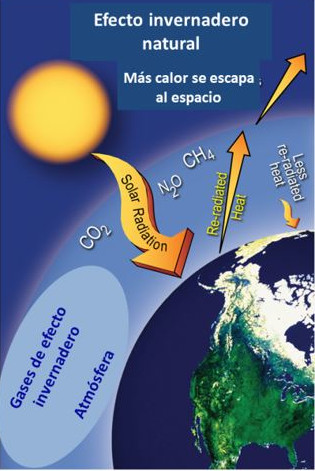
\includegraphics[scale=0.6]{Imagenes/Efecto_Invernadero_02.jpg}
\end{figure}
 
\subsection{Gases de efecto invernadero.}

Los principales gases de efecto invernadero en la atmósfera incluyen:
\begin{enumerate}
\item Dióxido de carbono (CO2)

Es el principal gas de efecto invernadero y es liberado principalmente por la quema de combustibles fósiles (petróleo, gas natural y carbón), la deforestación y los cambios en el uso del suelo. También se produce de forma natural en procesos como la respiración de los organismos vivos y la descomposición de la materia orgánica.
\item Metano (CH4)

Se produce principalmente durante la producción y transporte de combustibles fósiles, la agricultura (a través de la digestión de rumiantes, el cultivo de arroz y la gestión de estiércol) y la descomposición de residuos orgánicos en vertederos. Aunque es menos abundante que el dióxido de carbono, tiene un potencial de calentamiento global mucho mayor en el corto plazo.
\item Óxidos de nitrógeno (NOx)

Se producen principalmente durante la combustión de combustibles fósiles, la quema de biomasa y la agricultura (a través de la aplicación de fertilizantes sintéticos y la gestión de residuos agrícolas). Los óxidos de nitrógeno también contribuyen a la formación de smog y la lluvia ácida.
\item Ozono (O3)

El ozono en la troposfera es un contaminante del aire y un gas de efecto invernadero. Se forma a partir de reacciones químicas entre los óxidos de nitrógeno y los compuestos orgánicos volátiles en presencia de luz solar. El ozono troposférico es un componente importante del smog y puede ser perjudicial para la salud humana y la vegetación.
\item Vapor de agua (H2O)

Aunque el vapor de agua es el gas de efecto invernadero más abundante en la atmósfera, su concentración está determinada principalmente por la temperatura y la humedad atmosférica. Aunque no es generado por actividades humanas de manera directa, el aumento de la temperatura debido a las emisiones de otros gases de efecto invernadero puede aumentar la cantidad de vapor de agua en la atmósfera, lo que amplifica el efecto invernadero.
\end{enumerate}
Estos gases son liberados naturalmente por procesos biológicos y geológicos. Así como por actividades humanas (acciones antropogénicas) como la quema de combustibles fósiles, la deforestación y la agricultura.
\begin{figure}[H]
    \centering
    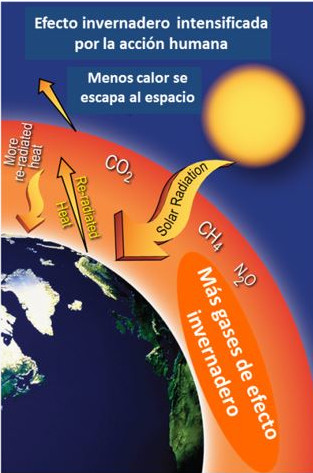
\includegraphics[scale=0.6]{Imagenes/Efecto_Invernadero_03.jpg}
\end{figure}

\section{Inversión térmica}
\subsection{¿Qué es la inversión térmica?}

Por lo regular a nivel de piso la temperatura es más caliente y las capas superiores son más templadas, predominando posteriormente aire frío.
\begin{figure}[H]
    \centering
    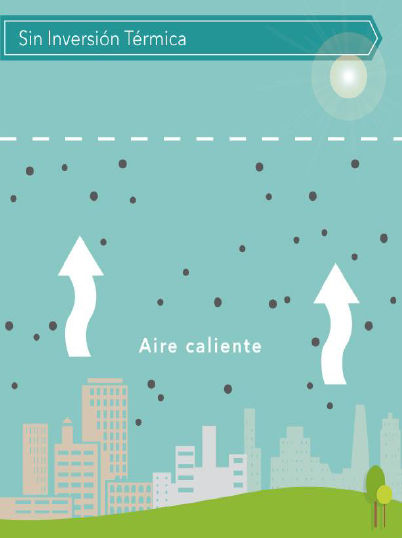
\includegraphics[scale=0.5]{Imagenes/Inversion_Termica_01.png}
\end{figure}
Cuando sucede el fenómeno de la inversión térmica se invierten las temperaturas: frío en la parte mas baja (capa más densa y pesada) y posteriormente aire caliente (capa menos densa y más ligera).

Estas capas actúan como una tapa que impide el movimiento ascendente del aire contaminado.
\begin{figure}[H]
    \centering
    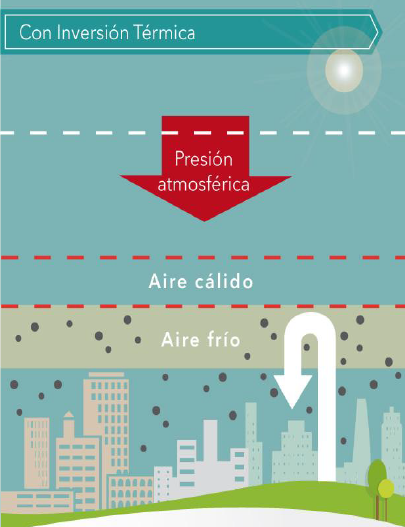
\includegraphics[scale=0.5]{Imagenes/Inversion_Termica_02.png}
\end{figure}
Debido a que se presenta una estabilidad del aire impidiendo cualquier tipo de intercambio vertical quedando atrapados los contaminantes. Arriba de la capa de aire caliente existe otra capa de aire frío a una mayor altura.

Algunas características clave de la inversión térmica:
\begin{enumerate}
\item Condiciones atmosféricas estables:

La inversión térmica suele ocurrir bajo condiciones atmosféricas estables, cuando hay poco movimiento vertical del aire y pocas nubes para retener el calor cerca de la superficie.
\item Capa de aire frío:

Durante una inversión térmica, una capa de aire frío se forma cerca de la superficie terrestre. Esto puede ocurrir porque el aire frío y denso se acumula en valles y áreas bajas.
\item Capa de aire cálido:

Encima de la capa de aire frío, hay una capa de aire más cálido. Este aire cálido actúa como una tapa que atrapa el aire frío debajo y evita que se mezcle con el aire más cálido de la atmósfera superior.
\item Efectos sobre la calidad del aire:

La inversión térmica puede tener efectos significativos sobre la calidad del aire, ya que puede atrapar contaminantes y partículas cerca de la superficie terrestre. Esto puede resultar en una acumulación de contaminantes, como smog y material particulado, lo que puede ser perjudicial para la salud humana y el medio ambiente.
\item Impacto en el clima local:

La inversión térmica puede afectar el clima local al influir en la circulación del aire y la dispersión de la humedad y los contaminantes. Puede causar neblina y niebla persistente en valles y áreas bajas, y también puede contribuir a la formación de eventos extremos, como heladas tardías en primavera.
\end{enumerate}

Es importante tener en cuenta que, si bien la inversión térmica puede tener algunos efectos negativos, también desempeña un papel importante en la regulación del clima y puede ser beneficiosa en ciertos contextos. Sin embargo, su impacto en la calidad del aire y la salud humana es una preocupación importante, especialmente en áreas urbanas donde la contaminación del aire puede ser un problema.

\subsection{Partículas suspendidas.}

Las partículas PM10 y PM2.5 son categorías de partículas suspendidas en el aire que tienen un diámetro aerodinámico menor o igual a 10 micrómetros (\unit{\micro\meter}) y 2.5 micrómetros, respectivamente. Estas partículas pueden tener diversas fuentes de origen tanto naturales como antropogénicas y son de gran importancia para la calidad del aire y la salud pública.

\begin{enumerate}
\item Partículas PM10 (partículas en suspensión con un diámetro menor o igual a 10 micrómetros):

Las partículas PM10 incluyen una amplia variedad de partículas en el aire, como polvo, polen, cenizas volcánicas, partículas de origen vegetal y animal, y partículas generadas por actividades humanas, como la quema de combustibles fósiles, la construcción, la minería y el transporte.

Estas partículas pueden ser inhaladas profundamente en los pulmones y pueden causar una variedad de problemas de salud, especialmente en personas con enfermedades respiratorias preexistentes, como asma, bronquitis crónica y enfermedad pulmonar obstructiva crónica (EPOC).

Las partículas PM10 también pueden contribuir a la formación de niebla y neblina, reducir la visibilidad y depositarse en superficies, causando contaminación de suelos y cuerpos de agua.
\item Partículas PM2.5 (partículas en suspensión con un diámetro menor o igual a 2.5 micrómetros):

Las partículas PM2.5 son aún más pequeñas que las PM10 y pueden penetrar más profundamente en los pulmones y el sistema respiratorio.

Estas partículas tienen una variedad de fuentes, incluidas las emisiones de vehículos de motor, la combustión de combustibles fósiles en plantas de energía y la calefacción residencial, la quema de biomasa (por ejemplo, madera y carbón), así como las actividades industriales y la agricultura.

Debido a su pequeño tamaño, las partículas PM2.5 pueden ser transportadas grandes distancias por el viento y pueden tener impactos adversos en la salud incluso en áreas lejanas a sus fuentes de emisión.

La exposición a largo plazo a altas concentraciones de partículas PM2.5 se ha asociado con una variedad de problemas de salud, incluyendo enfermedades cardíacas, accidentes cerebrovasculares, enfermedades respiratorias crónicas y cáncer de pulmón.
\end{enumerate}
\begin{figure}[H]
    \centering
    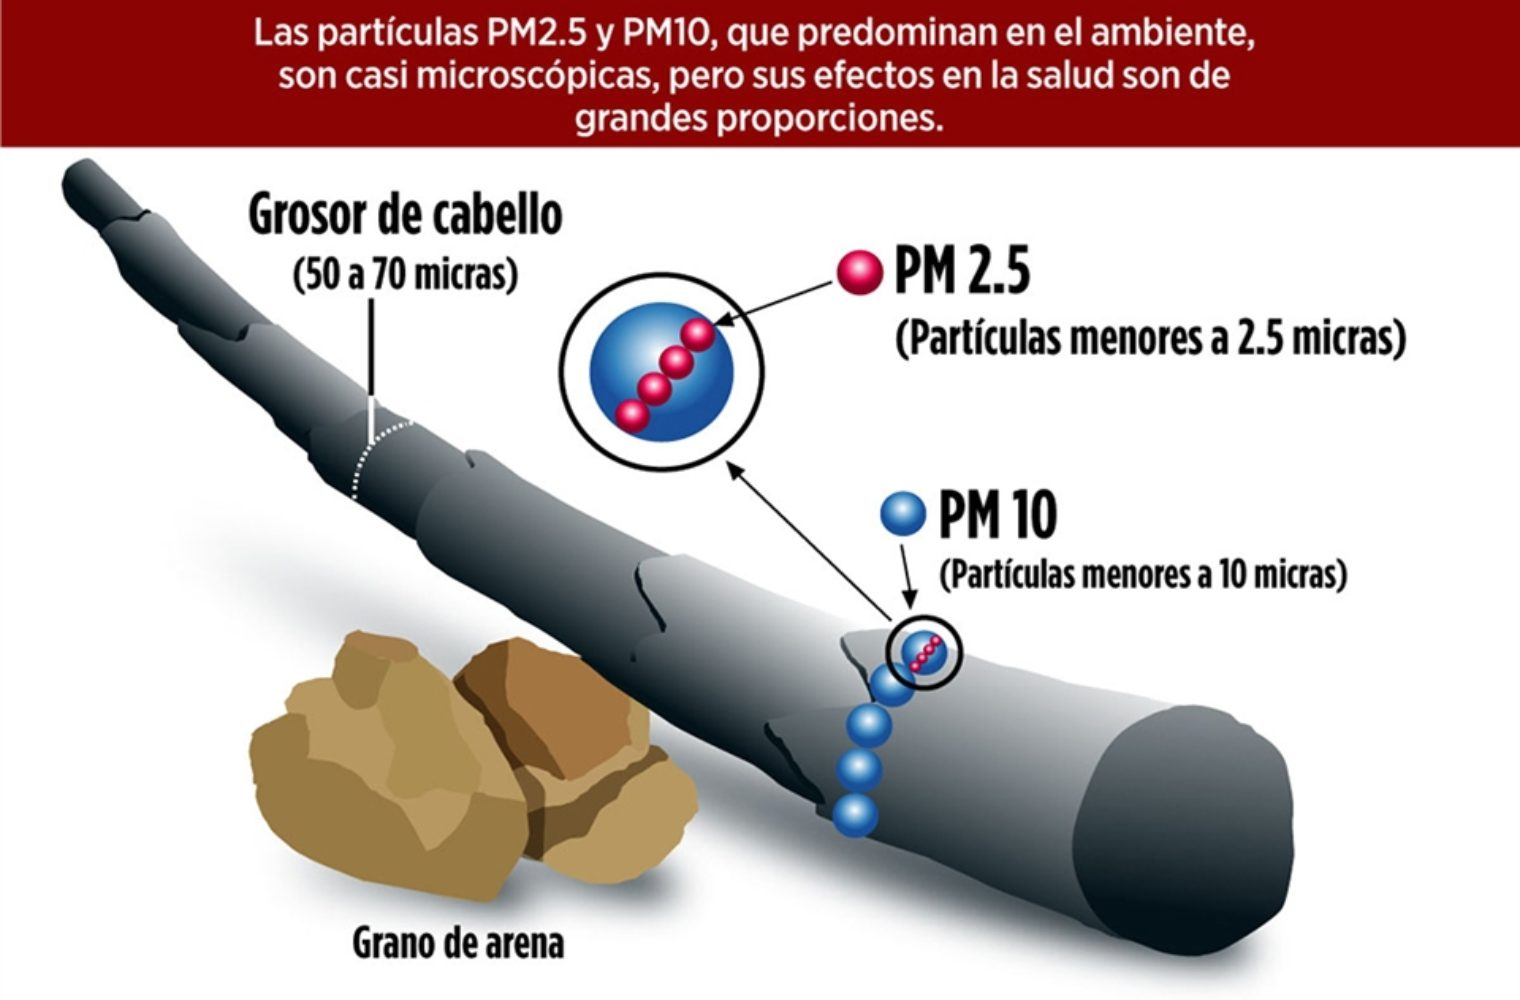
\includegraphics[scale=0.3]{Imagenes/Particulas_PM_01.jpg}
\end{figure}
Tanto las partículas PM10 como las PM2.5 son monitoreadas por agencias gubernamentales y organizaciones de salud pública en todo el mundo como indicadores clave de la calidad del aire y la contaminación atmosférica. La reducción de las emisiones de las fuentes de estas partículas y la implementación de medidas de control de la contaminación son fundamentales para proteger la salud humana y mejorar la calidad del aire en nuestras comunidades.

\end{document}